\documentclass[12pt]{article}
\usepackage{pdfpages}
\usepackage{eso-pic}
\usepackage{hyperref,url}
\usepackage{graphicx}
\graphicspath{{images/}}
\newcommand\tab[1][1cm]{\hspace*{#1}}

\begin{document}
\input{Titlu.tex}
\cleardoublepage

\newpage

\pagenumbering{arabic}
\setcounter{page}{1}
\setcounter{secnumdepth}{4}

\addtocontents{toc}{\protect\thispagestyle{empty}} % no page number on the table of contents page
\cleardoublepage

\section*{Lucrarea de laborator \#3}
\phantomsection

\section{Scopul lucrarii de laborator}
Realizarea unui simplu Web Site personal
Realizarea unui mockup corespunzatorul site-ului care urmeaza a fi realizat
Familiarizarea cu HTML si CSS
\section{Obiective}
Realizarea unui simplu Web Site personal si Mockupul.
Familiarizarea cu HTML si CSS.

\clearpage

\section{Screenshoturi la mockup}

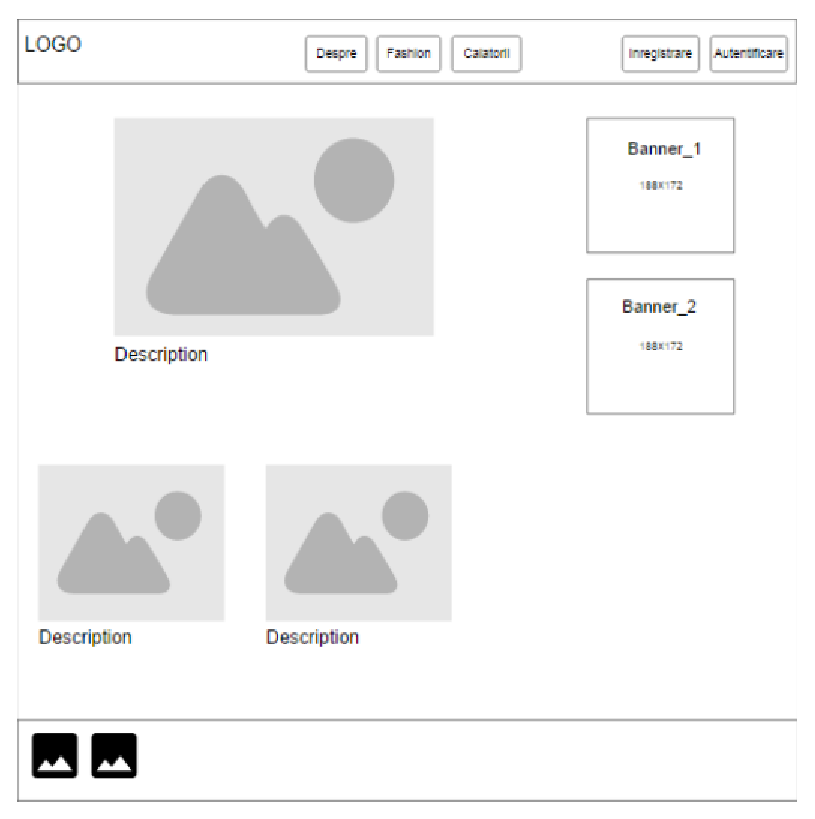
\includegraphics[width=\textwidth]{1.eps}
~\\
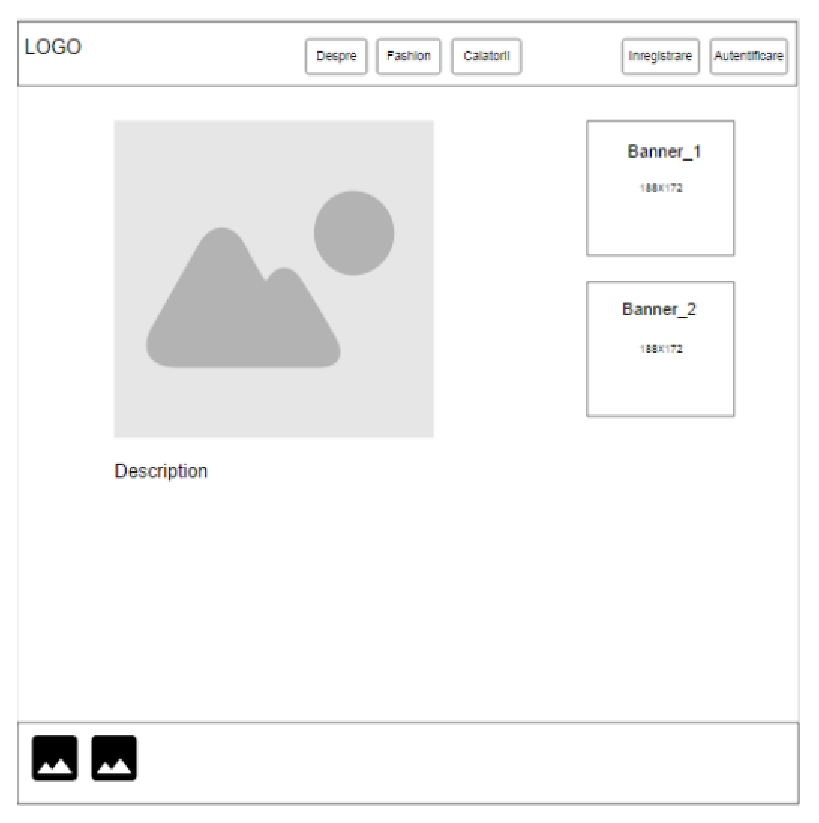
\includegraphics[width=\textwidth]{2.eps}
~\\
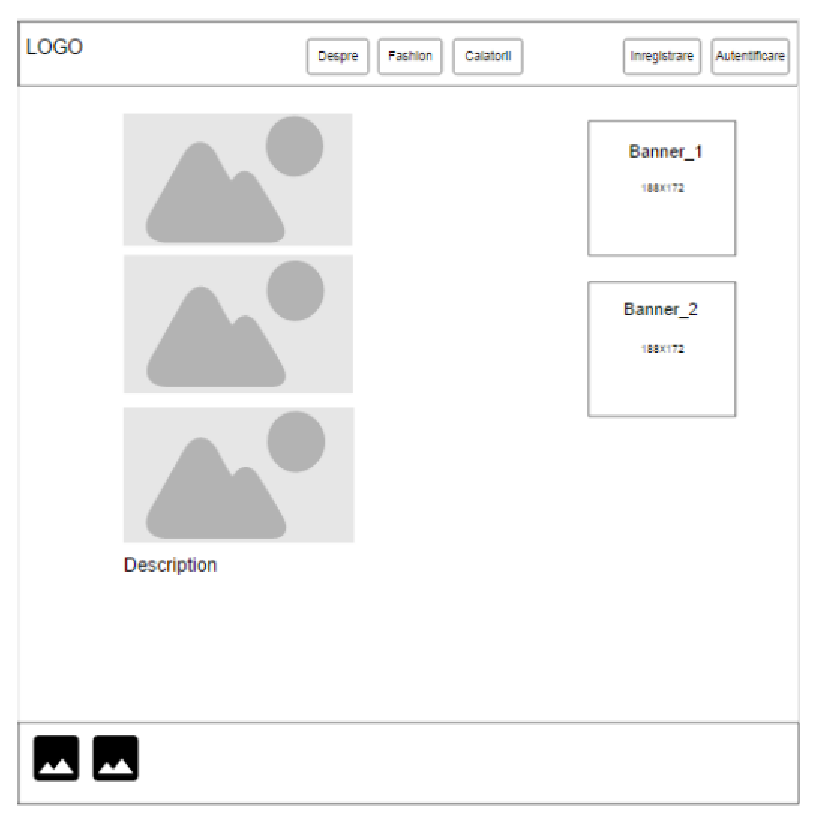
\includegraphics[width=\textwidth]{3.eps}
~\\
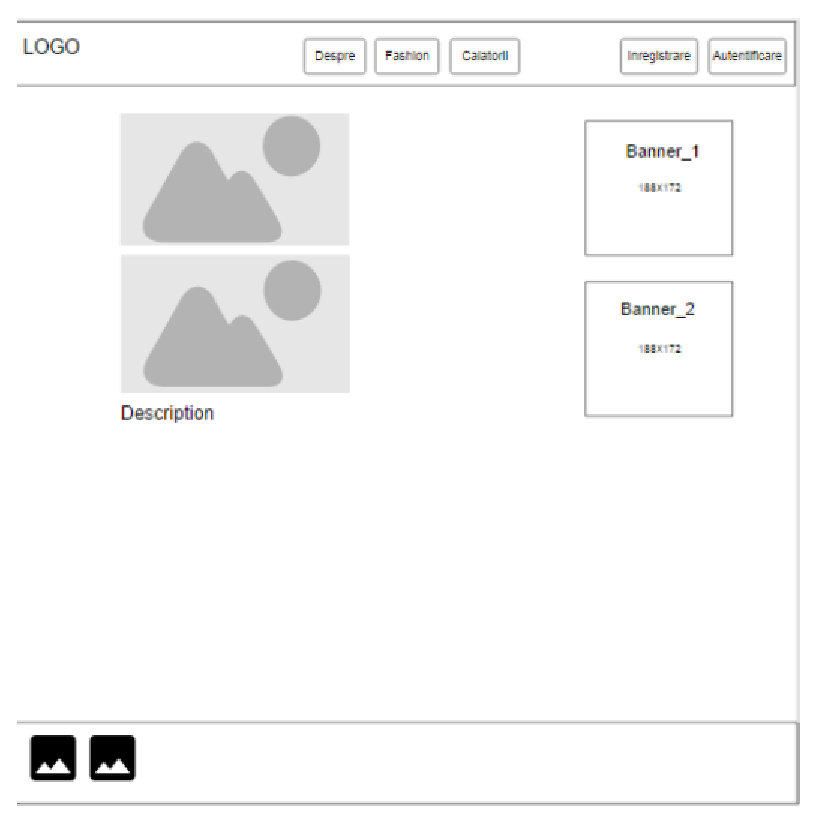
\includegraphics[width=\textwidth]{4.eps}
\clearpage

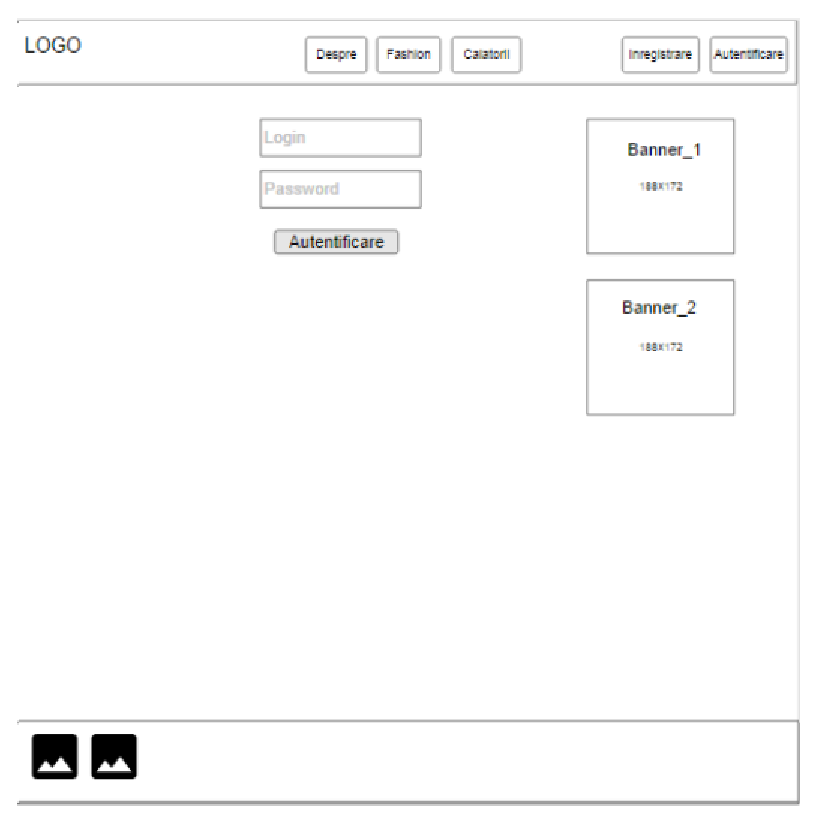
\includegraphics[width=\textwidth]{5.eps}
~\\
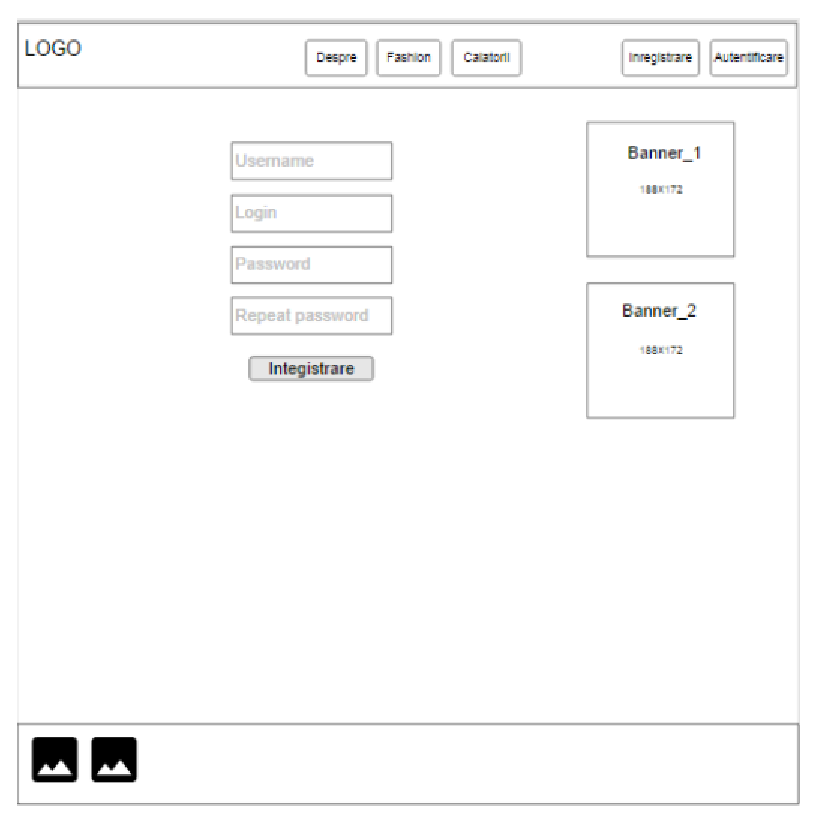
\includegraphics[width=\textwidth]{6.eps}
\clearpage
\section{Concluzie}
In aceasta lucrare de laborator am elaborat propriul web site. Intii de toate am elaborat mockup-ul pentru acest site care reprezinta un schelet si o baza pentru un viitor site si reprezinta un ghid pentru creare functionalitatii site-ului. Text editorul folosit este Notepad++ si limbajele de programare folosite si familiarizate sunt PHP,HTML si CSS. De asemenea am invatat cum sa gestionez pe blocuri site-ul pentru a nu scrie acelasi cod de mai multe ori, dar apelind codul scris o singura data. De asemenea am facut conexiune dintre site-ul creat si cu baza de date , si anume persoanele care se inregistreaza pe site se introduc in baza de date cu datele cu care s-a inregistrat,parola fiind criptata. Web development-ul este interesant prin documentatie, toturiale, si documentare.

\end{document}
